\section{Development of Phone Automation}
\label{sec:development}

The evolution of phone automation has been marked by significant technological advancements~\cite{kong2018automated}, particularly with the emergence of LLMs~\cite{radford2018gpt1,radford2019gpt2,brown2020gpt3,achiam2023gpt}. This section explores the historical development of phone automation, the challenges faced by traditional methods, and how LLMs have revolutionized the field.

\subsection{Phone Automation Before the LLM Era}
Before the advent of LLMs, phone automation was predominantly achieved through \textit{traditional technical methods}~\cite{kirubakaran2013mobile,azim2013targeted,amalfitano2014mobiguitar,linares2017continuous,kong2018automated,zhao2024dinodroid}. This subsection delves into the primary areas of research and application during that period, including automation testing, shortcuts, and Robotic Process Automation (RPA), highlighting their methodologies and limitations.

\subsubsection{Automation Testing}

Phone applications (apps) have become extremely popular, with approximately 1.68 million apps in the Google Play Store\footnote{\href{https://www.statista.com}{https://www.statista.com}.}. The increasing complexity of apps~\cite{hecht2015tracking} has raised significant concerns about app quality. Moreover, due to rapid release cycles and limited human resources, developers find it challenging to manually construct test cases. Therefore, various automated phone app testing techniques have been developed and applied, making phone automation testing the main application of phone automation before the era of large models~\cite{kirubakaran2013mobile,kong2018automated,linares2017continuous,zein2016systematic}. Test cases for phone apps are typically represented by a sequence of GUI events~\cite{jensen2013automated} to simulate user interactions with the app. The goal of automated test generators is to produce such event sequences to achieve high code coverage or detect bugs~\cite{zhao2024dinodroid}.

In the development history of phone automation testing, we have witnessed several key breakthroughs and advancements. Initially, random testing (e.g., Monkey Testing~\cite{machiry2013dynodroid}) was used as a simple and fundamental testing method, detecting application stability and robustness by randomly generating user actions. Although this method could cover a wide range of operational scenarios, its testing process lacked focus and was difficult to reproduce and pinpoint specific issues~\cite{kong2018automated}.

Subsequently, \textit{model-based testing}~\cite{amalfitano2012using,amalfitano2014mobiguitar,azim2013targeted} became a more systematic testing approach. It establishes a user interface model of the application, using predefined states and transition rules to generate test cases. This method improved testing coverage and efficiency, but the construction and maintenance of the model required substantial manual involvement, and updating the model became a challenge for highly dynamic applications.

With the development of machine learning techniques, \textit{learning-based} testing methods began to emerge~\cite{koroglu2018qbe,pan2020reinforcement,li2019humanoid,degott2019learning}. These methods generate test cases by analyzing historical data to learn user behavior patterns. For example, Humanoid \cite{li2019humanoid} uses deep learning to mimic human tester interaction behavior and uses the learned model to guide test generation like a human tester. However, this method relies on human-generated datasets to train the model and needs to combine the model with a set of predefined rules to guide testing.

Recently, \textit{reinforcement learning}~\cite{ladosz2022exploration} has shown great potential in the field of automated testing. DinoDroid~\cite{zhao2024dinodroid} is an example that uses Deep Q-Network (DQN)~\cite{fan2020theoretical} to automate testing of Android applications. By learning behavior models of existing applications, it automatically explores and generates test cases, not only improving code coverage but also enhancing bug detection capabilities. Deep reinforcement learning methods can handle more complex state spaces and make more intelligent decisions but also face challenges such as high training costs and poor model generalization capabilities~\cite{luo2024survey}.

\subsubsection{Shortcuts}

Shortcuts on mobile devices refer to predefined rules or trigger conditions that enable users to execute a series of actions automatically~\cite{bridle2006inducing,guerreiro2008mnemonical,kennedy2011use}. These shortcuts are designed to streamline interaction by reducing repetitive manual input. For instance, the Tasker app on the Android platform\footnote{\href{https://play.google.com}{https://play.google.com}.} and the Shortcuts feature on iOS\footnote{\href{https://support.apple.com}{https://support.apple.com}.} allow users to automate tasks like turning on Wi-Fi, sending text messages, or launching apps under specific conditions such as time, location, or events. These implementations leverage simple IF-THEN and manually-designed logic but are inherently limited in scope and flexibility. 


\subsubsection{Robotic Process Automation}

Robotic Process Automation(RPA) applications on phone devices aim to simulate human users performing repetitive tasks across applications~\cite{agostinelli2019research}. Phone RPA tools generate repeatable automation processes by recording user action sequences. These tools are used in enterprise environment to automate tasks such as data entry and information gathering, reducing human errors and improving efficiency, but they \textbf{struggle with dynamic interfaces and require frequent script updates}~\cite{pramod2022robotic,syed2020robotic}.

\subsection{Challenges of Traditional Methods}
\label{sebsec:challenges}

Despite the advancements made, traditional phone automation methods faced significant challenges that hindered further development. This subsection analyzes these challenges, including lack of generality and flexibility, high maintenance costs, difficulty in understanding complex user intentions, and insufficient intelligent perception, highlighting the need for new approaches.

\subsubsection{Limited Generality}

Traditional automation methods are often tailored to specific applications and interfaces, lacking adaptability to different apps and dynamic user environment~\cite{clarke2016therapeutic,li2017sugilite,patel2015home,asadullah2016overview}. For example, automation scripts designed for a specific app may not function correctly if the app updates its interface or if the user switches to a different app with similar functionality. This inflexibility makes it difficult to extend automation across various usage scenarios without significant manual reconfiguration.

These methods typically follow predefined sequences of actions and cannot adjust their operations based on changing contexts or user preferences. For instance, if a user wants an automation to send a customized message to contacts who have birthdays on a particular day, traditional methods struggle because they cannot dynamically access and interpret data from the contacts app, calendar, and messaging app simultaneously. Similarly, automating tasks that require conditional logic—such as playing different music genres based on the time of day or weather conditions—poses a challenge for traditional automation tools, as they lack the ability to integrate real-time data and make intelligent decisions accordingly~\cite{majeed2020intelligent,liu2023understanding}.

\subsubsection{High Maintenance Costs}

Writing and maintaining automation scripts require professional knowledge and are time-consuming and labor-intensive~\cite{kodali2019low,kodali2017low,moreira2023process,lamberton2017impact,meironke2022measure}. Taking RPA as an example, as applications continually update and iterate, scripts need frequent modifications. When an application's interface layout changes or functions are updated, RPA scripts originally written for the old version may not work properly, requiring professionals to spend considerable time and effort readjusting and optimizing the scripts~\cite{tripathi2018learning,ling2020intelligent,agostinelli2022reactive}.

The high entry barrier also limits the popularity of some automation features~\cite{le2020shortcut,roffarello2024trigger}. For example, Apple's Shortcuts \footnote{\href{https://support.apple.com}{https://support.apple.com}.} can combine complex operations, such as starting an Apple Watch fitness workout, recording training data, and sending statistical data to the user's email after the workout. However, setting up such a complex shortcut often requires the user to perform a series of complicated operations on the phone following fixed rules. This is challenging for ordinary users, leading many to abandon usage due to the complexity of manual script writing.

\subsubsection{Poor Intent Comprehension}

Rule-based and script-based systems can only execute predefined tasks or engage in simple natural language interactions~\cite{kepuska2018next,cowan2017can}. Simple instructions like "open the browser" can be handled using traditional natural language processing algorithms, but complex instructions like "open the browser, go to Amazon, and purchase a product" cannot be completed. These traditional systems are based on fixed rules and lack in-depth understanding and parsing capabilities for complex natural language~\cite{anicic2010rule,kang2013using,karanikolas2023large}.

They require users to manually write scripts to interact with the phone, greatly limiting the application of intelligent assistants that can understand complex human instructions. For example, when a user wants to check flight information for a specific time and book a ticket, traditional systems cannot accurately understand the user's intent and automatically complete the series of related operations, necessitating manual script writing with multiple steps, which is cumbersome and requires high technical skills.

\subsubsection{Weak Screen GUI Perception}

Different applications present a wide variety of GUI elements, making it challenging for traditional methods like RPA to accurately recognize and interact with diverse controls~\cite{fu2024understanding,banerjee2013graphical,chen2018ui,brich2017exploring}. Traditional automation often relies on fixed sequences of actions targeting specific controls or input fields, exhibiting Weak Screen GUI Perception that limits their ability to adapt to variations in interface layouts and component types. For example, in an e-commerce app, the product details page may include dynamic content like carousels, embedded videos, or interactive size selection menus, which differ significantly from the simpler layout of a search results page. Traditional methods may fail to accurately identify and interact with the "Add to Cart" button or select product options, leading to unsuccessful automation of purchasing tasks.


Moreover, traditional automation struggles with understanding complex screen information such as dynamic content updates, pop-up notifications, or context-sensitive menus that require adaptive interaction strategies. Without the ability to interpret visual cues like icons, images, or contextual hints, these methods cannot handle tasks that involve navigating through multi-layered interfaces or responding to real-time changes. For instance, automating the process of booking a flight may involve selecting dates from a calendar widget, choosing seats from an interactive seat map, or handling security prompts—all of which require sophisticated perception and interpretation of the interface~\cite{zhang2024llamatouch}.

In phone automation, many apps do not provide open API interfaces, forcing solutions to rely directly on the GUI for triggering actions and retrieving information. Even when tools are used to parse the Android UI~\cite{wu2021screen}, non-standard controls often prevent accurate JSON parsing, further complicating automated testing and interaction. Additionally, because the GUI is a universal and consistent interface across apps regardless of their internal design, it naturally becomes the central focus of phone automation methods.

These limitations significantly impede the widespread application and deep development of traditional phone automation technologies. Without intelligent perception capabilities, automation cannot adapt to the complexities of modern app interfaces, which are increasingly dynamic and rich in interactive elements. This underscores the urgent need for new methods and technologies that can overcome these bottlenecks and achieve more intelligent, flexible, and efficient phone automation.

\begin{figure*}[!ht]
\centering
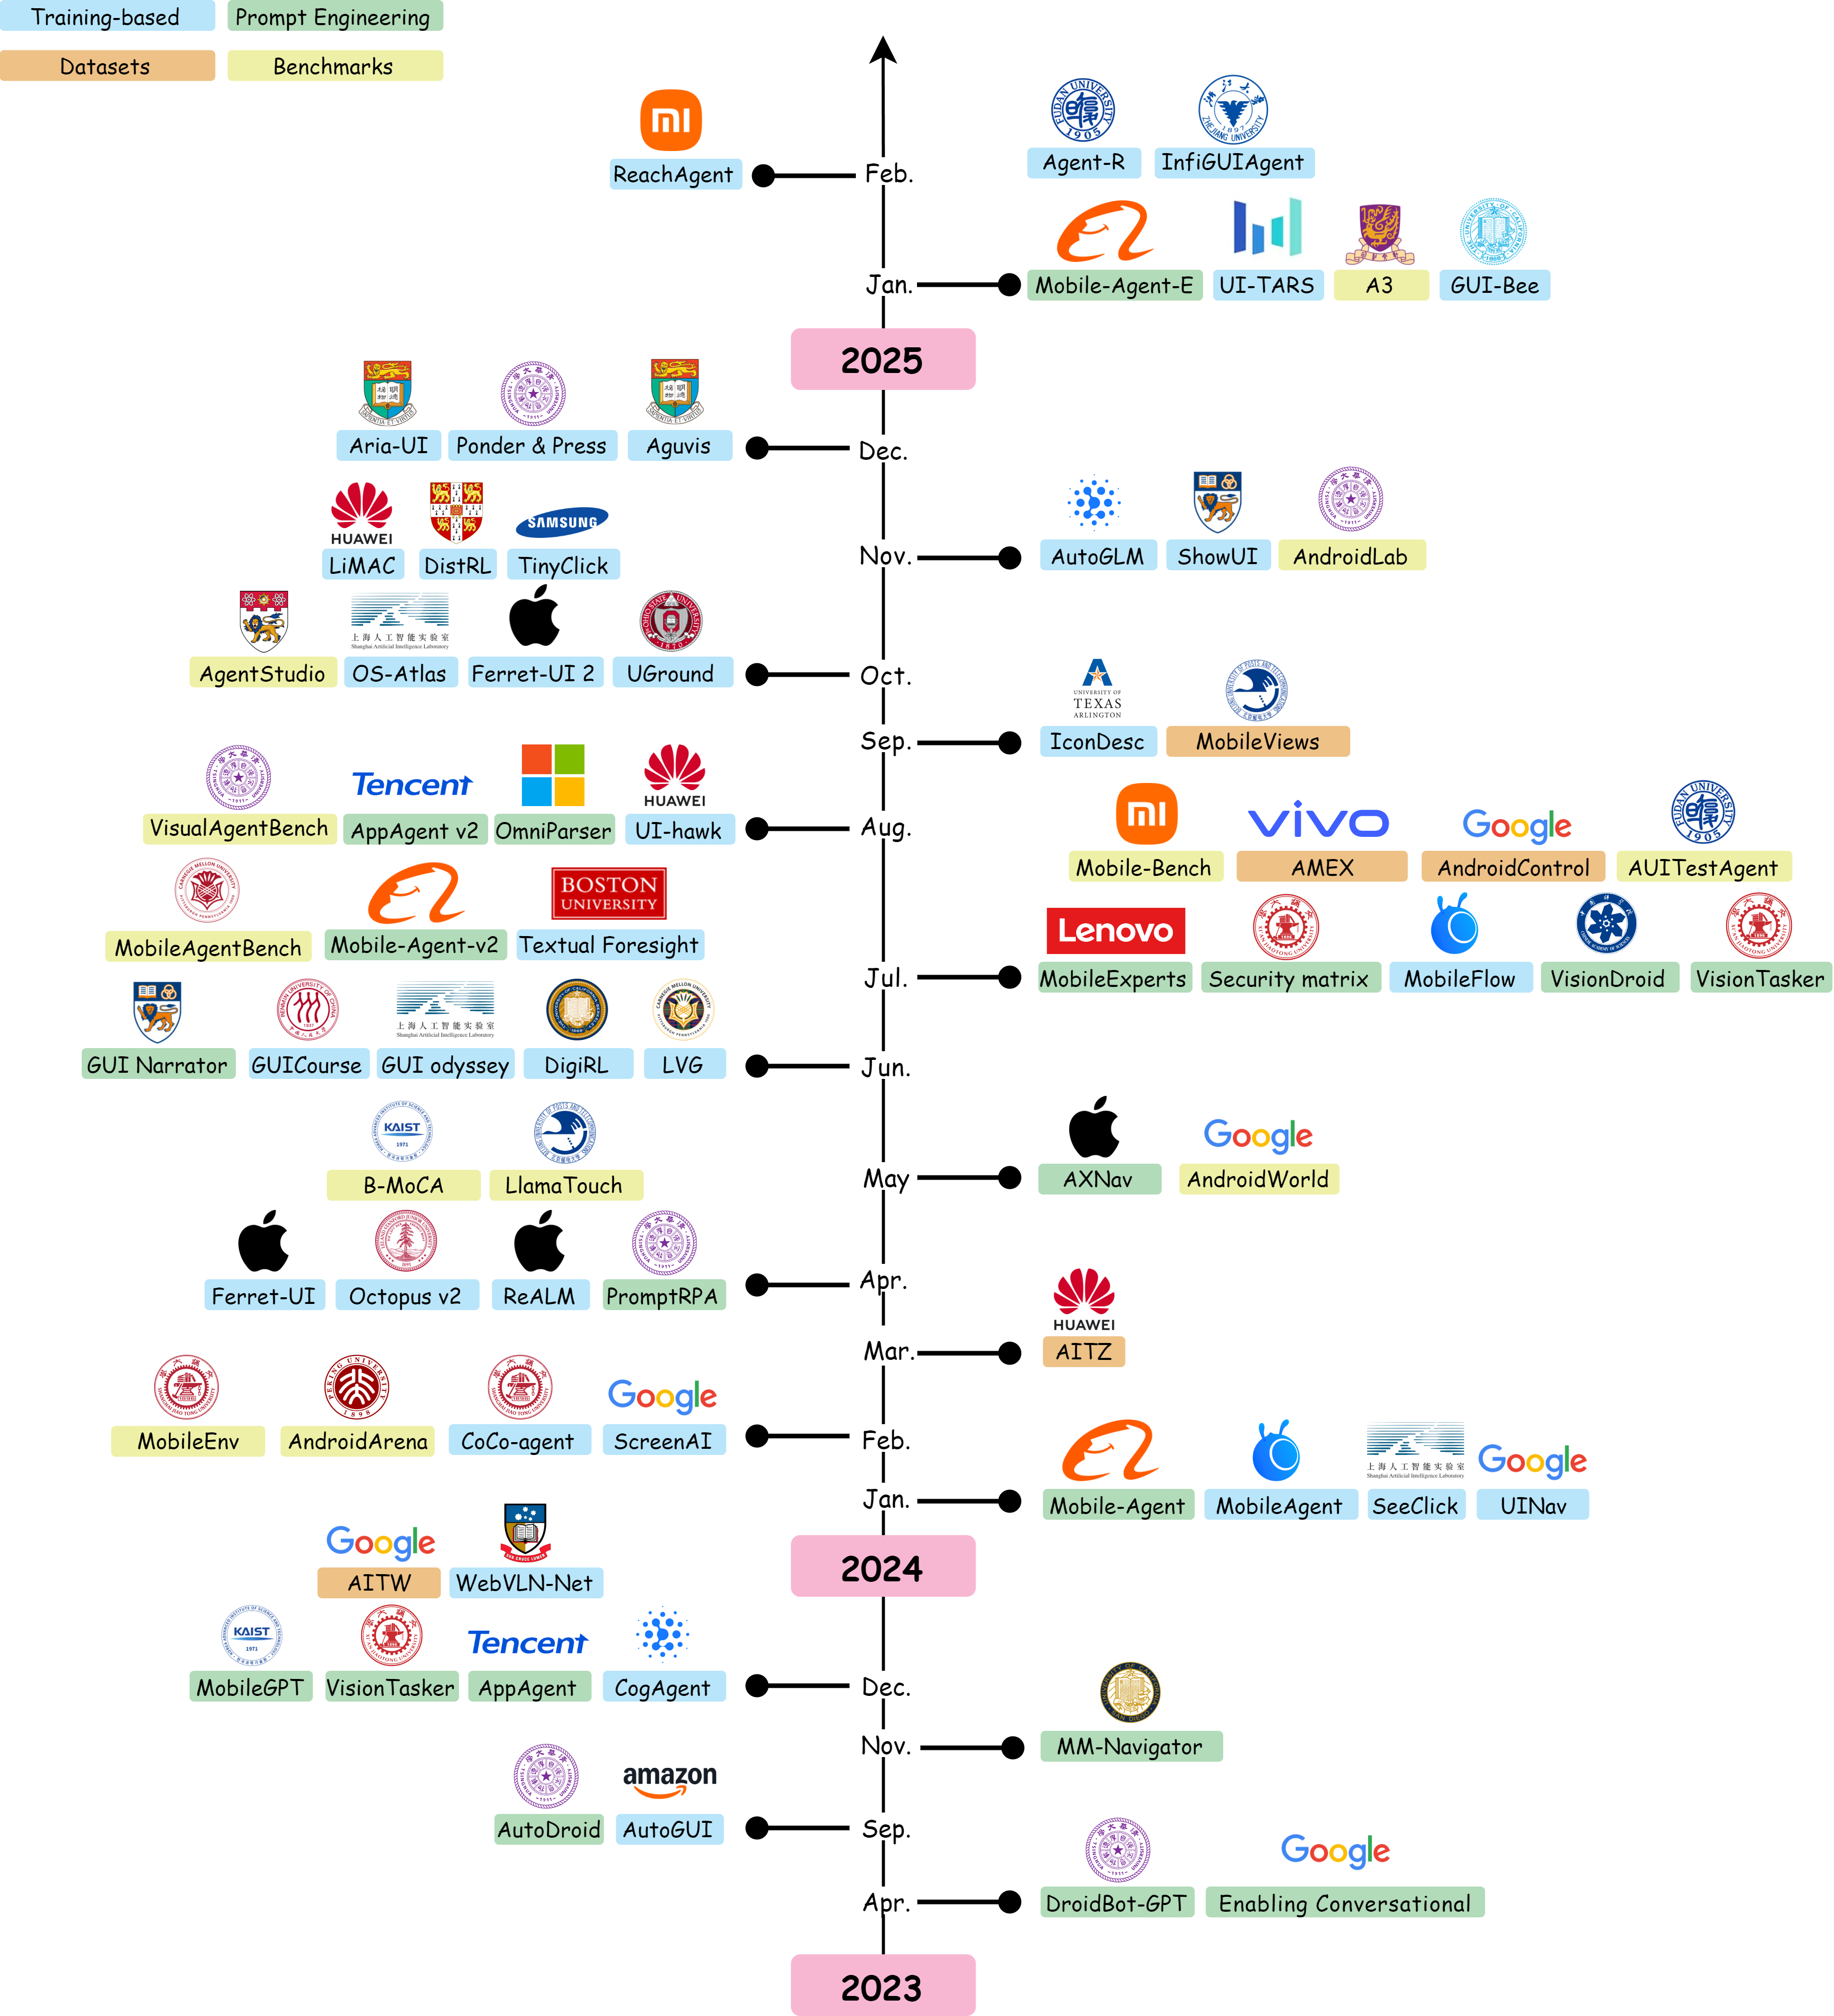
\includegraphics[width=0.95\linewidth]{figures/llm_phone_agent_milestones_optimized.png}
\caption{Milestones in the development of LLM-powered phone GUI agents. This figure divides advancements into four primary parts: \textbf{Prompt Engineering},  \textbf{Training-Based Methods}, \textbf{Datasets} and \textbf{Benchmarks}. Prompt Engineering leverages pre-trained LLMs by strategically crafting input prompts, as detailed in \S\ref{subsec:prompt_engineering}, to perform specific tasks without modifying model parameters. In contrast, Training-Based Methods, discussed in \S\ref{subsec:training_based}, involve adapting LLMs via supervised fine-tuning or reinforcement learning on GUI-specific data, thereby enhancing their ability to understand and interact with mobile UIs.}
\label{fig:llm_phone_agent_milestones}
\end{figure*}

\subsection{LLMs Boost Phone Automation}
\label{subsec:llms_boost_automation}

The advent of LLMs has marked a significant shift in the landscape of phone automation, enabling more dynamic, context-aware, and sophisticated interactions with mobile devices. As illustrated in Figure~\ref{fig:llm_phone_agent_milestones}, the research on LLM-powered phone GUI agents has progressed through pivotal milestones, where models become increasingly adept at interpreting multimodal data, reasoning about user intents, and autonomously executing complex tasks. This section clarifies how LLMs address traditional limitations and examines why \emph{scaling laws} can further propel large models in phone automation.
As will be detailed in \S\ \ref{sec:models} and \S\ \ref{sec:datasets_and_benchmarks}, LLM-based solutions for phone automation generally follow two routes: (1) \emph{Prompt Engineering}, where \emph{pre-trained} models are guided by carefully devised prompts, and (2) \emph{Training-Based Methods}, where LLMs undergo additional optimization on GUI-focused datasets. The following subsections illustrate how LLMs mitigate the core challenges of traditional phone automation—ranging from \emph{contextual semantic understanding} and \emph{GUI perception} to \emph{reasoning and decision making}—and briefly highlight the role of \emph{scaling laws} in enhancing these capabilities.



\noindent\textbf{Scaling Laws in LLM-Based Phone Automation.}
Scaling laws—originally observed in general-purpose LLMs, where increasing model capacity and training data yields emergent capabilities~\cite{brown2020language,kaplan2020scaling,hagendorff2023machine}—have similarly begun to manifest in phone GUI automation. As datasets enlarge and encompass more diverse apps, usage scenarios, and user behaviors, recent findings~\cite{cheng2024seeclick,chen2024guicourse,lu2024guiodyssey,pawlowski2024tinyclick} show consistent gains in step-by-step automation tasks such as clicking buttons or entering text. This data scaling not only captures broader interface layouts and device contexts but also reveals latent “emergent” competencies, allowing LLMs to handle more abstract, multi-step instructions. Empirical evidence from \emph{in-domain} scenarios~\cite{li2024androidcontrol} further underscores how expanded coverage of phone apps and user patterns systematically refines automation accuracy. In essence, as model sizes and data complexity grow, phone GUI agents exploit these scaling laws to bridge the gap between user intent and real-world GUI interactions with increasing efficiency and sophistication.


\noindent\textbf{Contextual Semantic Understanding.}
LLMs have transformed natural language processing for phone automation by learning from extensive textual corpora~\cite{vaswani2017attention,brown2020language,radford2018improving,devlin2018bert,wen2024autodroid,zhang2023appagent}. This training captures intricate linguistic structures and domain knowledge~\cite{karanikolas2023large}, allowing agents to parse multi-step commands and generate context-informed responses. MobileAgent~\cite{wang2024mobileagentv1}, for example, interprets user directives like scheduling appointments or performing transactions with high precision, harnessing the Transformer architecture~\cite{vaswani2017attention} for efficient encoding of complex prompts. Consequently, phone GUI agents benefit from stronger natural language grounding, bridging user-intent gaps once prevalent in script-based systems.


\noindent\textbf{Screen GUI with Multi-Modal Perception.}
Screen GUI perception in earlier phone automation systems typically depended on static accessibility trees or rigid GUI element detection, which struggled to adapt to changing app interfaces. Advances in LLMs, supported by large-scale multimodal datasets~\cite{zhao2023survey,chang2024survey,minaee2024large}, allow models to unify textual and visual signals in a single representation. Systems like UGround~\cite{gou2024navigating}, Ferret-UI~\cite{you2024ferret}, and UI-Hawk~\cite{zhang2024ui-hawk} excel at grounding natural language descriptions to on-screen elements, dynamically adjusting as interfaces evolve. Moreover, SeeClick~\cite{cheng2024seeclick} and ScreenAI~\cite{baechler2024screenai} demonstrate that learning directly from screenshots—rather than purely textual metadata—can further enhance adaptability. By integrating visual cues with user language, LLM-based agents can respond more flexibly to a wide range of UI designs and interaction scenarios.


\noindent\textbf{Reasoning and Decision Making.}
LLMs also enable advanced reasoning and decision-making by combining language, visual context, and historical user interactions. Pre-training on broad corpora equips these models with the capacity for complex reasoning~\cite{wang2023can,yuan2024advancing}, multi-step planning~\cite{song2023llm,valmeekam2023planning}, and context-aware adaptation~\cite{talukdar2024improving,koike2024outfox}. MobileAgent-V2~\cite{wang2024mobileagentv2}, for instance, introduces a specialized planning agent to track task progress while a decision agent optimizes actions. Auto-GUI~\cite{zhang2023youautoui} applies a multimodal chain-of-action approach that accounts for both previous and forthcoming steps, and SteP~\cite{sodhi2024step} uses stacked LLM modules to solve diverse web tasks. Similarly, MobileGPT~\cite{lee2023exploremobilegpt} leverages an app memory system to minimize repeated mistakes and bolster adaptability. Such architectures demonstrate higher success rates in complex phone operations, reflecting a new level of autonomy in orchestrating tasks that previously demanded handcrafted scripts.


Overall, LLMs are transforming phone automation by reinforcing semantic understanding, expanding multimodal perception, and enabling sophisticated decision-making strategies. The scaling laws observed in datasets like AndroidControl~\cite{li2024androidcontrol} reinforce the notion that a larger volume and diversity of demonstrations consistently elevate model accuracy. As these techniques mature, LLM-driven phone GUI agents continue to redefine how users interact with mobile devices, ultimately paving the way for a more seamless and user-centric automation experience.


\subsection{Emerging Commercial Applications}

The integration of LLMs has enabled novel commercial applications that leverage phone automation, offering innovative solutions to real-world challenges. This subsection highlights several prominent cases, presented in chronological order based on their release dates, where LLM-based GUI agents are reshaping user experiences, improving efficiency, and providing personalized services.


\noindent\textbf{Apple Intelligence.}
On June 11, 2024, Apple introduced its personal intelligent system, Apple Intelligence\footnote{\href{https://www.apple.com/apple-intelligence/}{https://www.apple.com/apple-intelligence/}.}, seamlessly integrating AI capabilities into iOS, iPadOS, and macOS. It enhances communication, productivity, and focus features through intelligent summarization, priority notifications, and context-aware replies. For instance, Apple Intelligence can summarize long emails, transcribe and interpret call recordings, and generate personalized images or “Genmoji.” A key aspect is on-device processing, which ensures user privacy and security. By enabling the system to operate directly on the user’s device, Apple Intelligence safeguards personal information while providing an advanced, privacy-preserving phone automation experience.


\noindent\textbf{vivo PhoneGPT.}
On October 10, 2024, vivo unveiled OriginOS 5\footnote{\href{https://www.vivo.com.cn/originos}{https://www.vivo.com.cn/originos}}, its newest mobile operating system, featuring an AI agent ability named PhoneGPT. By harnessing large language models, PhoneGPT can understand user instructions, preferences, and on-screen information, autonomously engaging in dialogues and detecting GUI states to operate the smartphone. Notably, it allows users to order coffee or takeout with ease and can even carry out a full phone reservation process at a local restaurant through extended conversations. By integrating the capabilities of large language models with native system states and APIs, PhoneGPT illustrates the great potential of phone GUI agents.


\noindent\textbf{Honor YOYO Agent.}
Released on October 24, 2024, the Honor YOYO Agent\footnote{\href{https://www.honor.com/cn/magic-os/}{https://www.honor.com/cn/magic-os/}.} exemplifies an phone automation assistant that adapts to user habits and complex instructions. With just one voice or text command, YOYO can automate multi-step processes—such as comparing prices to secure discounts when shopping, automatically filling out forms, ordering beverages aligned with user preferences, or silencing notifications during online meetings. By learning from user behaviors, YOYO reduces the complexity of human-device interaction, offering a more effortless and intelligent phone experience.


\noindent\textbf{Anthropic Claude Computer Use.}
On October 22, 2024, Anthropic unveiled the Computer Use feature for its Claude 3.5 Sonnet model\footnote{\href{https://www.anthropic.com/news/3-5-models-and-computer-use}{https://www.anthropic.com/news/3-5-models-and-computer-use}}. This feature allows an AI agent to interact with a computer as if a human were operating it, observing screenshots, moving the virtual cursor, clicking buttons, and typing text. Instead of requiring specialized environment adaptations, the AI can “see” the screen and perform actions that humans would, bridging the gap between language-based instructions and direct computer operations. Although initial performance is still far below human proficiency, this represents a paradigm shift in human-computer interaction. By teaching AI to mimic human tool usage, Anthropic reframes the challenge from “tool adaptation for models” to “model adaptation to existing tools.” Achieving balanced performance, security, and cost-effectiveness remains an ongoing endeavor.


\noindent\textbf{Zhipu.AI AutoGLM.}
On October 25, 2024, Zhipu.AI introduced AutoGLM~\cite{liu2024autoglm}, an intelligent agent that simulates human operations on smartphones. With simple text or voice commands, AutoGLM can like and comment on social media posts, purchase products, book train tickets, or order takeout. Its capabilities extend beyond mere API calls—AutoGLM can navigate interfaces, interpret visual cues, and execute tasks that mirror human interaction steps. This approach streamlines daily tasks and demonstrates the versatility and practicality of LLM-driven phone automation in commercial applications.


These emerging commercial applications—from Apple’s privacy-focused on-device intelligence to vivo’s PhoneGPT, Honor’s YOYO agent, Anthropic’s Computer Use, and Zhipu.AI’s AutoGLM—showcase how LLM-based agents are transcending traditional user interfaces. They enable more natural, efficient, and personalized human-device interactions. As models and methods continue to evolve, we can anticipate even more groundbreaking applications, further integrating AI into the fabric of daily life and professional workflows.
